\fig{fv:s3:interval}{平衡所需摩擦随外力改变，正负上限分别对应两种滑动趋势}{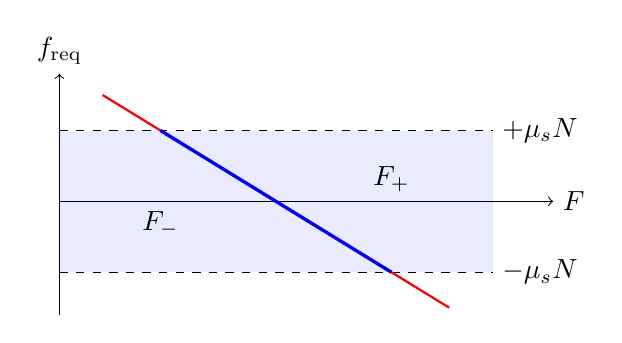
\begin{tikzpicture}[x=1.1cm,y=.9cm]
\fill[blue!8](0,-1)rectangle(5,1);\draw[->](0,0)--(5.7,0)node[right]{$F$};\draw[->](0,-1.6)--(0,1.8)node[above]{$f_{\rm req}$};
\draw[dashed](0,1)--(5,1)node[right]{$+\mu_sN$};\draw[dashed](0,-1)--(5,-1)node[right]{$-\mu_sN$};
\draw[red,thick](.5,1.5)--(4.5,-1.5);\draw[blue,very thick](1.167,1)--(3.833,-1);
\node[below]at(1.167,0){$F_-$};\node[above]at(3.833,0){$F_+$};
\end{tikzpicture}}
图\ref{fv:s3:interval}先由平衡方程求带符号的 $f_{\rm req}(F)$，再检查它是否落在允许带 $[-\mu_sN,\mu_sN]$内。蓝色线段对应整个可平衡区间，只有两端才达到极限摩擦。穿过横轴时摩擦方向改变，但物体仍可静止。若 $N$也随 $F$改变，允许带的边界会变成曲线或斜线，应联立完整不等式，不能沿用固定宽度的示意带。
